\chapter{Fundamentação Teórica}
\label{cap:fundamentacao-teorica}

% Alguns autores preferem fazer uma ``fundamentação teórica'' no segundo capítulo, outros, preferem fazer uma ``revisão da literatura''. Entretanto, isto é particular de cada trabalho e o autor deve escolher o título mais adequado para o capítulo. Consultar o orientador é importante para determinar o título apropriado.

% Evite começar da seção secundária, ou seja, não passe direto do título do capítulo para o título da seção secundária. Escreva um texto para introduzir as seções subsequentes. Lembre-se de utilizar primeira letra maiúscula quando estiver se referindo a um objeto com numeração específica como capítulo, seção, subseção, figura, tabela, quadro, equação, normalmente, se escreve a primeira letra maiúscula da palavra do objeto seguido do \textit{label}. Por exemplo, a Seção \ref{sec:citacoes} explica como fazer citações bibliográficas. Observe no código fonte deste texto como foi feita a referência cruzada. Isso permite enumerar a seção do modo automático o que facilita caso novas seções sejam criadas.  

Neste capítulo será introduzido a definição de sistemas embarcados, bem como alguns de seus tipos, diferenças arquiteturais e quais aplicações se encaixam melhor a cada um desses tipos de sistema. Em seguida, será apresentado a definição de \textit{Dataloggers} e possíveis aplicações





\section{Sistemas Embarcados}\label{sec:definicao_sistemas_embarcados}

% O processamento de informações até o fim dos anos 1980 era normalmente associado aos grandes computadores nos centros de dados, contudo, com a miniaturização dos componentes eletrônicos, isso passou a ser possível também com os computadores pessoais, que são utilizados principalmente para tarefas de escritório,


Sistemas computacionais são normalmente associados a grandes computadores de centros de processamento de dados, computadores de mesa e afins. Contudo, devido a miniaturização de componentes eletrônicos, esses sistemas puderam ser reduzidos ao ponto de fazerem parte da construção de diversos produtos do cotidiano. Impressoras, máquinas registradoras, controles remotos são alguns exemplos desses produtos. Dessa forma, para sistemas computacionais que são parte integrante de um produto ou ferramenta é dado a denominação de sistemas embarcados \cite{vahid2001embedded}.

Para atingir esse objetivo, contudo, um sistema embarcado possui um hardware com limitações de tamanho, consumo energético e poder de processamento para que a aplicação em que é utilizado seja viável. Essas limitações, contudo, fazem com que esse hardware  não possua a mesma padronização que o hardware utilizado em computadores pessoais, o que faz não só com que diversos tipos existam, como também torna difícil realizar um levantamento para se conhecer todos os tipos de componentes que compõem esse tipo de hardware \cite{marwedel2021embedded}. 

Contudo, à partir de características comuns aos sistemas embarcados, é possível definir que ele deve possuir uma estrutura básica que compreende uma unidade de processamento de informações, interfaces de entrada e saída de dados para que possam interagir com o ambiente, memórias para armazenamento de dados, interfaces de comunicação e uma unidade de fornecimento de energia elétrica. 


\section{Tecnologias de sistemas embarcados}


A unidade de processamento de um sistema embarcado é composta por um dispositivo processador de informações que é responsável por receber e tratar os dados do ambiente de acordo com as especificações da aplicação. Contudo, existem dispositivos que podem ser utilizados sendo eles os seguintes:


% \begin{itemize}
    \subsection{Processadores de propósito geral } São dispositivos que podem ser utilizados em diversas aplicações devido sua capacidade de ser programável, possuírem um grande número de instruções disponíveis para  uso e executam pode executar mais de um programa. Com esse tipo de dispositivo, o tempo de de criação e desenvolvimento de um sistema embarcado é menor, mas o custo unitário e o consumo de energia que uma aplicação que o use teria podem ser altos demais;
    
    \subsection{Processadores especializados } São dispositivos que também são programáveis, mas que possuem um conjunto de instruções otimizado para uma determinada classe de aplicações, o que leva a um custo maior de desenvolvimento. Apesar disso,  dependendo da aplicação pode se obter uma boa performance de processamento, consumo e tamanho da aplicação final. Alguns exemplos desse tipo de processadores são o microcontrolador e o \gls{DSP}. Aquele é um \gls{CI} que possui integrado não só uma \gls{CPU}, memória \gls{RAM} e interfaces de entrada e saída, mas também periféricos como \gls{UART}, \gls{I2C} e \gls{SPI}. É otimizado para aplicações de controle devido seu número de interfaces e periféricos, mas não é capaz de processar um grande volume de dados ou lidar com cálculos complexos que demandem uma solução rápida.
    
    Para essa tarefa é utilizado o \gls{DSP}, que pode ser tido como uma forma especializada de microcontrolador voltado para processamento de sinais. Possui características arquiteturais que o permitem realizar operações matemáticas, em particular adição e multiplicação, mais rápido que um microcontrolador comum, sendo normalmente utilizado em aplicações de telefonia ou para processamento de áudio e/ou vídeo.
    
    
    \subsection{Processadores dedicados } São dispositivos que não podem ser programados e são construídos de forma a atender uma aplicação especifica. Possuem a melhor performance e o menor consumo do gênero, mas apresentam um maior custo de desenvolvimento e produção porque uma vez que são construídos, não se pode alterar suas funcionalidades. Exemplos desse tipo de processadores é o \gls{ASIC}, que é um \gls{CI} que possui todas a lógica necessária para execução das tarefas de uma aplicação implementadas fisicamente, não sendo assim possível alterar qualquer uma delas caso haja algum erro de implementação. 
    
    Contudo, ainda que classificado nessa categoria, há também o \gls{FPGA}, que é também um \gls{CI} com as mesmas propriedades do \gls{ASIC}, exceto que ao contrário desse, um \gls{FPGA} pode ter suas instruções implementadas modificadas. Isso é possível devido sua construção ser baseada em uma matriz de blocos lógicos reconfiguráveis que são ligados entre si por meio de conexões programáveis, permitindo assim a reimplementação da lógica para execução das tarefas da aplicação.
% \end{itemize}



\section{System-On-A-Chip}

Um dos desafios da criação e produção de sistemas embarcados é a utilização do menor número de \gls{CI}s possível para atender as especificações de uma aplicação, assim, a possibilidade de se usar um único chip que satisfizesse essa necessidade seria a melhor solução. Isso é possível com o uso de um \gls{SOC}, um circuito integrado que é formado por diversos módulos que compõe um sistema computacional. \cite{hamacher2011computer}s

Além dos módulos básicos, \gls{CPU}, \gls{RAM} e interfaces de entrada/saída, esse tipo de circuito integrado pode possuir módulos de processamento de sinais, módulos de comunicações sem fio e mais. Embora mais caro que microcontroladores ou \gls{DSP}s já discutidos, dependendo da aplicação, a comodidade de se possuir tantos módulos em um único circuito integrado se mostra vantajosa.



\section{Características Comuns}

Sistemas embarcados, além das limitações de recursos, possuem algumas características que são comuns a todos independentemente da aplicação. A primeira delas é a forma de interação com o ambiente, que devido a falta de suporte a telas e teclados assim como computadores pessoais, que se dá por meio de sensores e atuadores conectados ao hardware do sistema embarcado. Essa forma de interação faz com que esses dispositivos sejam tipicamente sistemas reativos, que são sistemas que estão em constante interação com o ambiente esperando por algum estímulo e executam um conjunto de instruções bem definidas quando são detectados.

Além disso, devido suas características, um sistema embarcado é dedicado somente para uma aplicação, não sendo possível executar instruções de outras aplicações no mesmo dispositivo. Dessa forma, o sistema que controla um forno micro-ondas executa somente as instruções relativas ao controle dos circuitos do forno de acordo com determinadas condições, não sendo possível executar um outro um programa de um jogo, por exemplo. 



\section{Desafios de projeto}

O projeto de um sistema enfrenta muitas desafios e problemas não só por causa da limitação de recursos disponíveis para uso, como também na forma como a aplicação deve interagir com o ambiente. Um dos desafios comuns é criar um sistema que atenda a requisitos de dependabilidade.

Segundo \citeonline{marwedel2021embedded}, um sistema embarcado atinge a dependabilidade quando consegue executar suas funcionalidades com uma alta probabilidade e sem causar nenhum dano. Essa propriedade é necessária devido aos impactos imediatos que um sistema embarcado pode ter em um determinado ambiente. Assim, para se atingir esse estado é preciso que os seguintes aspectos sejam atendidos:

\begin{itemize}

    \item \textbf{Segurança da informação} - Define-se como a preservação da confidencialidade, integridade e disponibilidade da informação processada;
    
    \item \textbf{Confidencialidade} - Um dos aspectos da segurança da informação, pode ser definido como a propriedade da informação de não estar disponível para entidades, pessoas ou processos não autorizados;
    
    \item \textbf{Operação segura} - É definida como a ausência de riscos inaceitáveis, danos físicos ou à saúde das pessoas, direta ou indiretamente devido algum dano ao ambiente;
    
    \item \textbf{Confiabilidade} - Probabilidade de que um sistema não irá falhar dentro de um determinado período de tempo;
    
    \item \textbf{Reparabilidade} - Probabilidade que um sistema falho tem de ser reparado dentro de um determinado período de tempo;
    
    \item \textbf{Disponibilidade} - Pode ser definido como a probabilidade de um sistema estar disponível.
    
    
\end{itemize}

\newpage

Além da dependabilidade, outro desafio importante no desenvolvimento de um sistema embarcado é a criação de um dispositivo que faça o uso eficiente de recursos computacionais. Alguns desses recursos que devem ser considerados para análise durante a criação do sistema embarcado são:

\begin{itemize}

    \item Memória (\gls{RAM});
    \item Espaço de código;
    \item Ciclos de processador ou velocidade;
    \item Uso eficiente de bateria (economia de energia);
    \item Periféricos do processador.
    
\end{itemize}   


Deve ser feito assim, a escolha de qual desses recursos priorizar, de acordo com a aplicação. Para isso, pode-se realizar trocas da quantidade disponível de um desses recursos por outro, por exemplo, para priorizar o uso eficiente de baterias pode ser reduzido a velocidade do processador para que ele consumo menos energia na execução das suas funções. Contudo, mesmo com essa possibilidade, nem todos os recursos são passíveis de serem otimizados em detrimento de outros. \cite{white2011making}

%%%%%%%%%%% Sensores e Atuadores %%%%%%%%%%%%%%%%%%
% Sistemas embarcados precisam ser capazes de receber, processar e responder estímulos do ambientes mas diferentemente de computadores de mesa, celulares ou afins, não podem contar com o uso de teclados e telas para fazer essa interação. Dessa forma, um sistema embarcado interage com o ambiente que está inserido por meio do uso de sensores e atuadores. 

% \section{Dataloggers}\label{sec:datalogger}

% Um \textit{Datalogger} é um dispositivo de funcionamento autônomo, que conta com sensores, memória interna e é capaz de realizar e disponibilizar a leitura de uma ou mais variáveis do ambiente e armazená-lo por um determinado período de tempo que pode ser de dias, meses ou até anos. Contudo, para atender a esse requisito, a taxa de amostragem dessas variáveis é limitada a escala de segundos, do contrário sua memória interna seria ocupada totalmente em um curto período de tempo.


% \section{\textit{Data Acquisition Systems} - DAQs}

\if{0}
    % Esta frase mostra como citar um livro sobre descargas atmosféricas \cite{rakov2003lightning}. Também podem ser citados \textit{sites} como \citeonline{elat2015densidade}. Você precisa escrever o código da referência no arquivo "referencia.bib" dentro da pasta "elementos-pos-textuais". Veja esse, onde estão alguns exemplos que já foram testados.        

    Referenciando outro livro \cite{LangtangenLogg2017}. Texto texto texto texto texto texto texto texto texto texto texto texto texto texto texto texto texto texto texto. Texto texto texto texto texto texto texto texto texto texto texto texto texto texto texto texto texto texto texto. Texto texto texto texto texto texto texto texto texto texto texto texto texto texto texto texto texto texto texto. Texto texto texto texto texto texto texto texto texto texto texto texto texto texto texto texto texto texto texto.

    Referenciando outro site \cite{secretaria1999}. Texto texto texto texto texto texto texto texto texto texto texto texto texto texto texto texto texto texto texto. Texto texto texto texto texto texto texto texto texto texto texto texto texto texto texto texto texto texto texto. Texto texto texto texto texto texto texto texto texto texto texto texto texto texto texto texto texto texto texto. Texto texto texto texto texto texto texto texto texto texto texto texto texto texto texto texto texto texto texto. Citando uma norma \cite{NBR10520:2002}.
        
    Citação de duas referências que concordam entre si \cite{Almeida2018,Gondim2017}. Texto texto texto texto texto texto texto texto texto texto texto texto texto texto texto texto texto texto texto. Texto texto texto texto texto texto texto texto texto texto texto texto texto texto texto texto texto texto texto. Texto texto texto texto texto texto texto texto texto texto texto texto texto texto texto texto texto texto texto. Texto texto texto texto texto texto texto texto texto texto texto texto texto texto texto texto texto texto texto texto texto texto texto texto texto texto. Citando um manual \cite{manuais1989}. 
        
    Outro tipo de citação é a citação literal ou direta com mais de três linhas. Este tipo de citação deve ser destacada com recuo de $4~cm$ da margem esquerda com letra menor (tamanho 10), sem aspas e com espaçamento simples.  Para exemplificar esse tipo de citação, considere a afirmação de \citeonline{feitosa2016}:
    \begin{citacao}
        A cultura é o processo através do qual o homem cria o algo onde antes imperava o nada. Esse algo é toda complexidade de criações simbólicas, de sentidos e significados que damos às coisas e ao mundo. Um ``algo'' que não se sustenta se não se entender os processos culturais como mecanismos de mediação entre nós e os fenômenos. Assim, mais do que apenas um elemento da comunicação, a mediação é, por excelência, cultural. As diversas modalidades de mediação são apenas sotaques diferenciados dessa mediação cultural. Assim é a mediação informacional.
    \end{citacao}
        
    A afirmação do parágrafo anterior também pode ser reproduzida com a citação na final como mostra o exemplo a seguir: 
    \begin{citacao}
        A cultura é o processo através do qual o homem cria o algo onde antes imperava o nada. Esse algo é toda complexidade de criações simbólicas, de sentidos e significados que damos às coisas e ao mundo. Um “algo” que não se sustenta se não se entender os processos culturais como mecanismos de mediação entre nós e os fenômenos. Assim, mais do que apenas um elemento da comunicação, a mediação é, por excelência, cultural. As diversas modalidades de mediação são apenas sotaques diferenciados dessa mediação cultural. Assim é a mediação informacional. \cite{feitosa2016}.
    \end{citacao}
        
%Mais exemplos e opções de citações podem ser encontradas em:
%        https://en.wikibooks.org/wiki/LaTeX/Bibliography_Management
%        https://github.com/cfgnunes/latex-cefetmg/blob/master/latex-cefetmg/03-elementos-pos-textuais/apendices.tex            

\section{Inserindo figuras}\label{sec:figuras}
    
    A Figura \ref{fig:reitoria} apresenta a fotografia da reitoria da Universidade Federal do Ceará. Observe a estrutura do código para ver como inserir figuras. No título, comece especificando o tipo de figura. Por exemplo, fotografia, desenho, diagrama, fluxograma, gráfico e etc. O espaçamento entre linhas no título é de $1~pt$ (espaçamento simples), apenas a primeira letra da frase é maiúscula. As demais palavras são escritas com letra maiúsculas somente quando são nomes próprios e não há ponto final. 
    
    As margens do título da figura são delimitadas pelo tamanho da figura. Por isso, procure ajustar o tamanho da figura para preencher a largura delimitada pelas margens esquerda e direita da página que possui $16~cm$ de largura. Não esqueça de indicar fonte da figura. O autor deve evitar deixar figuras pequenas menores do que $7~cm$ de largura.
    
    A posição da figura deve ser o mais próximo logo após ter sido chamada no texto (a figura nunca deve aparecer antes de ter sido anunciada no texto). 
    
    %troque h pelo b ou t para mudar a posição da figura.
 	\begin{figure}[h!] 
   	    \captionsetup{width=16cm}%Da mesma largura que a figura
		\Caption{\label{fig:reitoria} Fotografia da reitoria da Universidade Federal do Ceará}
		\UFCfig{}{
			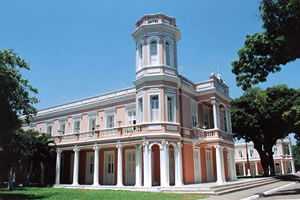
\includegraphics[width=16cm]{figuras/exemplo-1}
		}{
			\Fonte{\citeonline{UFC2012}.}
		}	
	\end{figure}
	
    Texto1 texto texto texto texto texto texto texto texto texto texto texto texto texto texto texto texto texto texto texto texto texto texto texto texto texto texto texto texto texto texto texto texto texto texto texto texto texto texto texto texto texto texto texto texto1.

    Texto2 texto texto texto texto texto texto texto texto texto texto texto texto texto texto texto texto texto texto. Texto texto texto texto texto texto texto texto texto texto texto texto texto texto texto texto texto texto texto2.

    Texto3 texto texto texto texto texto texto texto texto texto texto texto texto texto texto texto texto texto texto. Texto texto texto texto texto texto texto texto texto texto texto texto texto texto texto texto texto texto texto3.

    Texto4 texto texto texto texto texto texto texto texto texto texto texto texto texto texto texto texto texto texto. Texto texto texto texto texto texto texto texto texto texto texto texto texto texto texto texto texto texto texto4.

    A Figura \ref{fig:sondas} Texto texto texto texto texto texto texto texto texto texto texto texto texto texto texto texto texto texto texto. Texto texto texto texto texto texto texto texto texto texto texto texto texto texto texto texto texto texto texto3.

	\begin{figure}[h!]
		\centering
		\captionsetup{width=14cm}%Da mesma largura que a figura
		\Caption{\label{fig:sondas} Gráfico da Atmosfera Superior}	
		\UFCfig{}{
			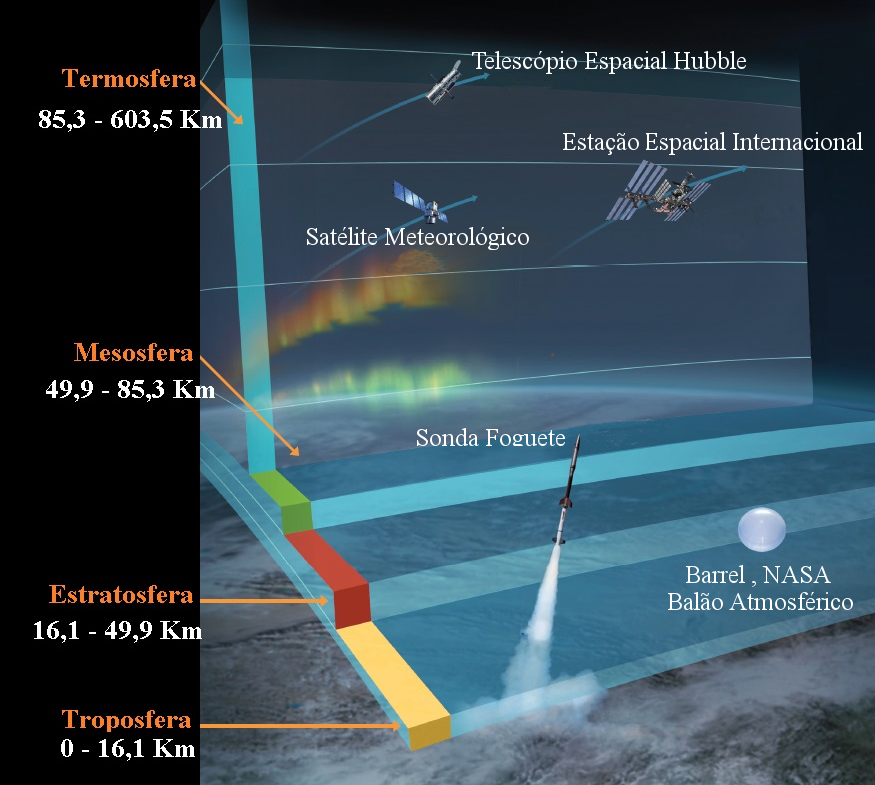
\includegraphics[width=14cm]{figuras/sondas}
		}{
			\Fonte{adaptado da \citeonline{NASA2016}.}}	
	\end{figure}

    Texto5 texto texto texto texto texto texto texto texto texto texto texto texto texto texto texto texto texto texto texto texto texto texto texto texto texto texto texto texto texto texto texto texto texto texto texto texto texto texto texto texto texto texto texto texto5.

    Texto6 texto texto texto texto texto texto texto texto texto texto texto texto texto texto texto texto texto texto texto texto texto texto texto texto texto texto texto texto texto texto texto texto texto texto texto texto texto texto texto texto texto texto texto texto5.

    Texto7 texto texto texto texto texto texto texto texto texto texto texto texto texto texto texto texto texto texto texto texto texto texto texto texto texto texto texto texto texto texto texto texto texto texto texto texto texto texto texto texto texto texto texto texto texto texto texto texto texto texto texto texto texto texto texto texto texto texto texto texto texto texto texto6.

    Evite terminar seções, capítulos e etc com figura. Procure escrever mais.

\section{Inserindo tabelas}\label{sec:tabelas}
    
    A Tabela \ref{tab:exemplo-1}... texto texto texto texto texto texto texto texto texto texto texto texto texto texto texto texto texto texto texto. Texto texto texto texto texto texto texto texto texto texto texto texto texto texto texto texto texto texto texto.
	
	\begin{table}[!h]
	\captionsetup{width=7cm}%Deixe da mesma largura que a tabela
	\Caption{\label{tab:exemplo-1} Um Exemplo de tabela alinhada que pode ser longa ou curta}%
	\IBGEtab{}{%
		\begin{tabular}{ccc}
			\toprule
			Nome & Nascimento & Documento \\
			\midrule \midrule
			Maria da Silva & 11/11/1111 & 111.111.111-11 \\
			Maria da Silva & 11/11/1111 & 111.111.111-11 \\
			Maria da Silva & 11/11/1111 & 111.111.111-11 \\
			\bottomrule
		\end{tabular}%
	}{%
	\Fonte{o autor.}%
	\Nota{esta é uma nota, que diz que os dados são baseados na
		regressão linear.}%
	\Nota[Anotações]{uma anotação adicional, seguida de várias outras.}%
    }
    \end{table}

	%\begin{table}[h!]	
	%	\centering
	%	\Caption{\label{tab:exemplo-1} Exemplo de tabela}	
	%	\UFCtab{}{
	%		\begin{tabular}{cll}
	%			\toprule
	%			Ranking & Exon Coverage & Splice Site Support \\
	%			\midrule \midrule
	%			E1 & Complete coverage by a single transcript & Both splice sites\\
	%			E2 & Complete coverage by more than a single transcript & Both splice sites\\
	%			E3 & Partial coverage & Both splice sites\\
	%			E4 & Partial coverage & One splice site\\
	%			E5 & Complete or partial coverage & No splice sites\\
	%			E6 & No coverage & No splice sites\\
	%			\bottomrule
	%		\end{tabular}
	%	}{
	%	\Fonte{elaborado pelo autor.}
	%}
	%\end{table}

\subsection{Exemplo de subseção} \label{sec:ex_sec}
	
    Texto texto texto texto texto texto texto texto texto texto texto texto texto texto texto texto texto texto texto texto texto texto texto texto texto texto texto texto texto texto texto texto texto texto texto texto texto texto texto texto texto texto texto texto texto.

    %acrlong{DATASUS},\acrlong{DNV},\acrlong{DO},\acrlong{ESF},\acrlong{IBGE},\acrlong{MFC},\acrlong{MI},\acrlong{MS},\acrlong{NV},\acrlong{ODM},\acrlong{OI},\acrlong{OMS},\acrlong{ONU},\acrlong{PNI},\acrlong{PSF},\acrlong{RIPSA},\acrlong{RN},\acrlong{SIM},\acrlong{SINASC},\acrlong{SUS},\acrlong{TMI},\acrlong{TMMFC}


    \begin{alineascomponto}
	    \item Integer non lacinia magna. Aenean tempor lorem tellus, non sodales nisl commodo ut
	    \item Proin mattis placerat risus sit amet laoreet. Praesent sapien arcu, maximus ac fringilla efficitur, vulputate faucibus sem. Donec aliquet velit eros, sit amet elementum dolor pharetra eget
	    \item Integer eget mattis libero. Praesent ex velit, pulvinar at massa vel, fermentum dictum mauris. Ut feugiat accumsan augue, et ultrices ipsum euismod vitae
	    \begin{subalineascomponto}
		    \item Integer non lacinia magna. Aenean tempor lorem tellus, non sodales nisl commodo ut
		    \item Proin mattis placerat risus sit amet laoreet.
	    \end{subalineascomponto}
    \end{alineascomponto}

\subsection{Uso de siglas} \label{sec:siglas}

    Para utilizar siglas, primeiro defina a sigla no arquivo "lista-de-abreviaturas-e-siglas"~ dentro da pasta "1-pre-textuais" com o comando 
    \begin{verbatim}
        \newacronym{ABNT}{ABNT}{Associação Brasileira de Normas Técnicas}
    \end{verbatim}
    Depois chame a sigla com o comando:
    \begin{verbatim}
        \gls{ABNT}
    \end{verbatim}
    Fica assim: \gls{ABNT}. A primeira vez que o comando é usado para uma determinada sigla, aparece o significado por extenso da sigla com a sua abreviação em seguida. A partir da segunda vez que o comando para uma determinada sigla é usado, aparace apenas a sigla. Por exemplo: \gls{ABNT}.  
    
    Veja o código fonte de outros exemplos: Teste de siglas \gls{TEST}, outros exemplos de siglas: \gls{DA}, \gls{MCEG}. 
    Repare que sempre as siglas estão sendo definidas primeiramente no arquivo ``lista-de-abreviaturas-e-siglas''.
\fi